\documentclass[12pt,a4paper]{article}

% ─── Page Layout ───────────────────────────────────────────────────────────────
\usepackage[a4paper, margin=0.8in, headheight=14pt]{geometry}

% ─── Fonts (XeLaTeX) ───────────────────────────────────────────────────────────
\usepackage{fontspec}
\usepackage{unicode-math}
\setmainfont{TeX Gyre Pagella}
\setmonofont[Scale=0.88]{TeX Gyre Cursor}
\setmathfont{Latin Modern Math}

% ─── Packages ──────────────────────────────────────────────────────────────────
\usepackage{xcolor}
\usepackage{colortbl}
\usepackage{titlesec}
\usepackage{enumitem}
\usepackage{tabularx}
\usepackage{booktabs}
\usepackage{array}
\usepackage{amsmath}
\usepackage{tikz}
\usetikzlibrary{shapes.geometric, arrows.meta, positioning, calc, fit, decorations.pathreplacing, patterns}
\usepackage{tcolorbox}
\tcbuselibrary{skins, breakable}
\usepackage{hyperref}
\usepackage{fancyhdr}
\usepackage{graphicx}
\usepackage{microtype}
\hyphenpenalty=10000
\exhyphenpenalty=10000
\sloppy
\usepackage{caption}
\usepackage{setspace}
\usepackage{multirow}
\usepackage{tocloft}

% ─── Q&A helper ────────────────────────────────────────────────────────────────
\newcommand{\Q}[1]{\textbf{#1}\par\noindent\ignorespaces}

% ─── Colour Palette ────────────────────────────────────────────────────────────
\definecolor{myred}{RGB}{196,30,58}
\definecolor{mydark}{RGB}{30,30,50}
\definecolor{mygreen}{RGB}{14,120,80}
\definecolor{myteal}{RGB}{0,130,140}
\definecolor{myamber}{RGB}{180,100,0}
\definecolor{mypurple}{RGB}{100,30,160}
\definecolor{mygray}{RGB}{246,247,249}
\definecolor{mgframe}{RGB}{180,185,200}
\definecolor{watermark}{RGB}{145,150,170}
\definecolor{hdrred}{RGB}{250,232,235}
\definecolor{hdrgreen}{RGB}{220,244,233}
\definecolor{hdrteal}{RGB}{220,242,244}
\definecolor{hdramber}{RGB}{253,242,215}
\definecolor{hdrpurple}{RGB}{238,228,255}
\definecolor{hdrgray}{RGB}{238,240,245}
\definecolor{rowalt}{RGB}{250,251,253}

% ─── Section Formatting ────────────────────────────────────────────────────────
\titleformat{\section}
  {\large\bfseries\color{myred}}{\thesection.}{0.5em}{}
  [\vspace{1pt}{\color{myred}\rule{\linewidth}{0.8pt}}]
\titleformat{\subsection}
  {\normalsize\bfseries\color{myteal}}{\thesubsection}{0.5em}{}
\titlespacing*{\section}{0pt}{18pt}{7pt}
\titlespacing*{\subsection}{0pt}{11pt}{4pt}

% ─── Paragraph ─────────────────────────────────────────────────────────────────
\setlength{\parindent}{0pt}
\setlength{\parskip}{4pt}

% ─── TOC Styling ───────────────────────────────────────────────────────────────
\renewcommand{\cfttoctitlefont}{\large\bfseries\color{myred}}
\renewcommand{\cftaftertoctitle}{\par\noindent{\color{myred}\rule{\linewidth}{0.8pt}}}
\setlength{\cftbeforetoctitleskip}{0pt}
\setlength{\cftaftertoctitleskip}{6pt}
\renewcommand{\cftsecfont}{\normalsize\bfseries\color{mydark}}
\renewcommand{\cftsecpagefont}{\normalsize\bfseries\color{mydark}}
\renewcommand{\cftsecleader}{\cftdotfill{\cftdotsep}}
\setlength{\cftbeforesecskip}{7pt}
\renewcommand{\cftsubsecfont}{\small\color{mydark}}
\renewcommand{\cftsubsecpagefont}{\small\color{mydark}}
\setlength{\cftbeforesubsecskip}{3pt}
\setlength{\cftsubsecindent}{1.4em}

% ─── Table helpers ─────────────────────────────────────────────────────────────
\renewcommand{\arraystretch}{1.45}
\setlength{\tabcolsep}{6pt}
\arrayrulecolor{mydark}
\newcolumntype{B}[1]{>{\small\bfseries\raggedright\arraybackslash}m{#1}}
\newcolumntype{Y}{>{\small\raggedright\arraybackslash}X}
\renewcommand{\tabularxcolumn}[1]{m{#1}}

% ─── Header / Footer ───────────────────────────────────────────────────────────
\pagestyle{fancy}
\fancyhf{}
\fancyhead[L]{\small\color{myred}\textbf{ES-CS301}\;\color{mydark}--- Data Structure \& Algorithms}
\fancyhead[R]{\small\color{myteal}\textbf{Module 1 Notes}}
\fancyfoot[C]{\small\color{mydark}\thepage}
\fancyfoot[R]{\small\color{watermark}\textit{\copyright\ Biraj}}
\renewcommand{\headrulewidth}{0.5pt}
\renewcommand{\footrulewidth}{0.3pt}

% ─── Hyperref ──────────────────────────────────────────────────────────────────
\hypersetup{
  colorlinks=true, linkcolor=myteal, urlcolor=myteal,
  pdfauthor={Biraj Sarkar (CGEC)},
  pdftitle={ES-CS301 --- Module 1 Notes: Introduction, Algorithm Analysis and Searching}
}

% ─── tcolorbox styles ──────────────────────────────────────────────────────────
\tcbset{
  tikzbox/.style={
    colback=mygray, colframe=mgframe, boxrule=0.6pt, arc=4pt,
    left=8pt, right=8pt, top=6pt, bottom=6pt,
    colbacktitle=mgframe, coltitle=mydark,
    fonttitle=\small\bfseries
  },
  defbox/.style={
    colback=hdrgreen, colframe=mygreen, boxrule=0.8pt, arc=4pt,
    left=9pt, right=9pt, top=6pt, bottom=6pt,
    colbacktitle=mygreen, coltitle=white,
    fonttitle=\small\bfseries
  },
  formulabox/.style={
    colback=hdrteal, colframe=myteal, boxrule=0.8pt, arc=4pt,
    left=9pt, right=9pt, top=7pt, bottom=7pt,
    colbacktitle=myteal, coltitle=white,
    fonttitle=\small\bfseries
  },
  examplebox/.style={
    colback=hdramber, colframe=myamber, boxrule=0.8pt, arc=4pt,
    left=9pt, right=9pt, top=6pt, bottom=6pt,
    colbacktitle=myamber, coltitle=white,
    fonttitle=\small\bfseries
  },
  masonbox/.style={
    colback=hdrpurple, colframe=mypurple, boxrule=0.8pt, arc=4pt,
    left=9pt, right=9pt, top=6pt, bottom=6pt,
    colbacktitle=mypurple, coltitle=white,
    fonttitle=\small\bfseries
  },
  exambox/.style={
    colback=hdrpurple, colframe=mypurple, boxrule=1pt, arc=5pt,
    left=10pt, right=10pt, top=8pt, bottom=8pt,
    colbacktitle=mypurple, coltitle=white,
    fonttitle=\bfseries,
    breakable, title after break={\textbf{Frequently Asked / Viva Questions (contd.)}}
  }
}

\tcbset{breakable}
\tcbset{after={\color{black}}}

% ─── TikZ styles ───────────────────────────────────────────────────────────────
\tikzset{
  circnode/.style={circle, draw=myteal, fill=hdrteal, inner sep=2pt, minimum size=6pt},
  block/.style={rectangle, draw=myteal, fill=hdrteal, text width=2.5cm, align=center, minimum height=0.9cm, font=\small, rounded corners=3pt, line width=0.7pt},
  redblock/.style={rectangle, draw=myred, fill=hdrred, text width=2.5cm, align=center, minimum height=0.9cm, font=\small\bfseries, rounded corners=3pt, line width=0.8pt},
  greenblock/.style={rectangle, draw=mygreen, fill=hdrgreen, text width=2.5cm, align=center, minimum height=0.9cm, font=\small, rounded corners=3pt, line width=0.7pt},
  arrow/.style={-Stealth, thick, color=mydark},
  redarrow/.style={-Stealth, thick, color=myred},
  line/.style={thick, color=mydark}
}

\begin{document}

% ─── Title Page ───────────────────────────────────────────────────────────────
\begin{center}
  {\LARGE\bfseries\color{myred} ES-CS301 --- Data Structure \& Algorithms}\\[5pt]
  {\normalsize\color{mydark} Semester III \quad$\bullet$\quad 3L:0T:4P \quad$\bullet$\quad 3 Credits}\\[3pt]
  {\normalsize\color{myteal}\textbf{Module 1 Exam Notes: Introduction, Algorithm Analysis and Searching}}\\[3pt]
  {\small\color{mydark} CGEC \;$|$\; B.Tech ECE (2023--27) \;$|$\; \textit{Biraj Sarkar}}
\end{center}
\vspace{2pt}
\noindent{\color{myred}\rule{\linewidth}{1.5pt}}
\vspace{2pt}

\hypersetup{linkcolor=mydark}
\tableofcontents
\hypersetup{linkcolor=myteal}
\newpage

% ───────────────────────────────────────────────────────────────────────────────
\section{Elementary Data Organizations and Terminologies}
% ───────────────────────────────────────────────────────────────────────────────

\begin{tcolorbox}[defbox, title={\textbf{Definition: Data Structure and Abstract Data Type (ADT)}}]
A \textbf{data structure} is a specialized mathematical or logical organization of data items alongside a set of well-defined operations, designed to facilitate efficient storage, retrieval, and algorithmic modification in computer memory.
\par\vspace{4pt}
An \textbf{Abstract Data Type (ADT)} is an axiomatic mathematical specification of a data structure that defines:
\begin{enumerate}[leftmargin=*, nosep]
  \item The domain of data elements stored, and
  \item The legal operations performed upon them together with their formal behavioral contracts,
\end{enumerate}
independent of any underlying hardware architecture, compiler implementation, or memory layout.
\end{tcolorbox}

\subsection{Basic Data Organization Terminologies}
Data items are structured hierarchically in memory from physical bits to logical models:
\begin{itemize}[leftmargin=*, itemsep=3pt]
  \item \textbf{Data Item:} A single unit of value (e.g., an integer or a character).
  \item \textbf{Elementary vs Group Data Item:} An elementary item cannot be decomposed further (e.g., student ID). A group item can be divided into sub-items (e.g., full name divided into first, middle, and last names).
  \item \textbf{Entity and Attribute:} An entity represents a concrete real-world object (e.g., an employee). An attribute is an observable property or characteristic of that entity (e.g., age, salary).
  \item \textbf{Record:} A composite collection of heterogeneous data attributes representing a single entity.
  \item \textbf{File:} A collection of structurally identical records representing an entity set.
\end{itemize}

\subsection{Taxonomy of Data Structures}
Data structures are classified across multiple functional dimensions:
\begin{enumerate}[leftmargin=*, itemsep=4pt]
  \item \textbf{Primitive vs Non-Primitive:} Primitive types are directly manipulated by underlying machine instructions (e.g., \texttt{int}, \texttt{float}, \texttt{char}, pointers). Non-primitive types are derived composite structures (e.g., arrays, lists, trees).
  \item \textbf{Linear vs Non-Linear:} In a linear data structure, elements form a strictly sequential 1-to-1 ordering where every element (except first and last) has a unique predecessor and successor (e.g., Array, Linked List, Stack, Queue). In non-linear data structures, elements exhibit hierarchical (1-to-many) or interconnected (many-to-many) relationships (e.g., Trees, Graphs).
  \item \textbf{Static vs Dynamic:} Static structures maintain a fixed memory allocation determined at compile time (e.g., static arrays). Dynamic structures allocate and deallocate physical memory blocks at runtime via system heaps (e.g., Linked Lists, dynamic BSTs).
  \item \textbf{Homogeneous vs Heterogeneous:} Homogeneous structures enforce identical data types for all elements (e.g., arrays). Heterogeneous structures permit dissimilar types (e.g., C \texttt{struct}, records).
  \item \textbf{Persistent vs Ephemeral:} Ephemeral structures destroy earlier versions upon modification; persistent structures preserve previous historical states after updates.
\end{enumerate}

\begin{tcolorbox}[tikzbox, title={\textbf{Structural Hierarchy and Taxonomy of Data Structures}}]
\centering
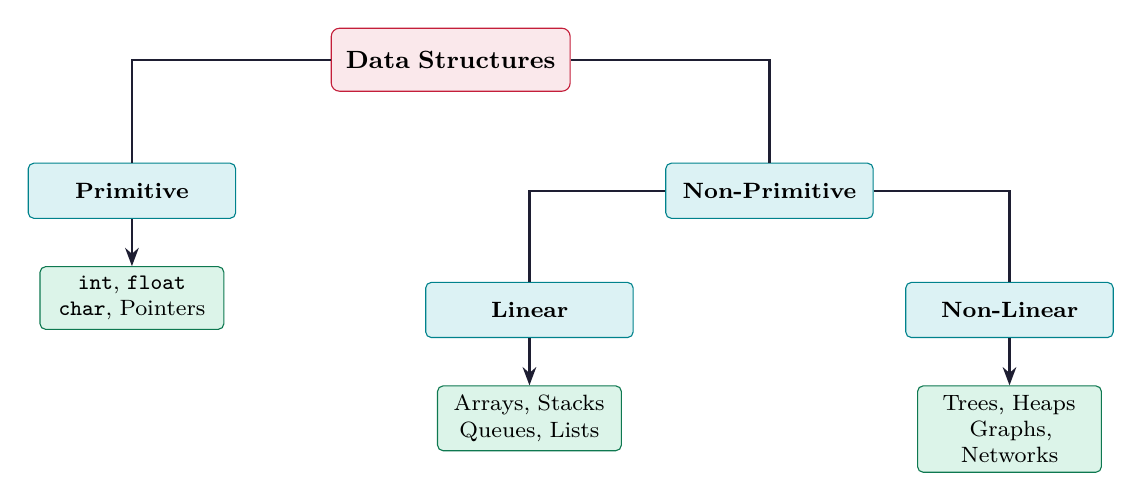
\begin{tikzpicture}[
  node distance=0.8cm and 0.6cm,
  every node/.style={font=\footnotesize},
  root/.style={rectangle, draw=myred, fill=hdrred, font=\small\bfseries, rounded corners=3pt, text width=2.8cm, align=center, minimum height=0.8cm},
  cat/.style={rectangle, draw=myteal, fill=hdrteal, font=\footnotesize\bfseries, rounded corners=2pt, text width=2.4cm, align=center, minimum height=0.7cm},
  leaf/.style={rectangle, draw=mygreen, fill=hdrgreen, rounded corners=2pt, text width=2.1cm, align=center, minimum height=0.65cm}
]
  \node[root] (ds) {Data Structures};
  \node[cat, below left=0.9cm and 1.2cm of ds] (prim) {Primitive};
  \node[cat, below right=0.9cm and 1.2cm of ds] (nonprim) {Non-Primitive};

  \draw[line] (ds) -| (prim);
  \draw[line] (ds) -| (nonprim);

  \node[leaf, below=0.6cm of prim] (p1) {\texttt{int}, \texttt{float}\\ \texttt{char}, Pointers};
  \draw[arrow] (prim) -- (p1);

  \node[cat, below left=0.8cm and 0.4cm of nonprim] (lin) {Linear};
  \node[cat, below right=0.8cm and 0.4cm of nonprim] (nonlin) {Non-Linear};

  \draw[line] (nonprim) -| (lin);
  \draw[line] (nonprim) -| (nonlin);

  \node[leaf, below=0.6cm of lin] (l1) {Arrays, Stacks\\ Queues, Lists};
  \node[leaf, below=0.6cm of nonlin] (nl1) {Trees, Heaps\\ Graphs, Networks};

  \draw[arrow] (lin) -- (l1);
  \draw[arrow] (nonlin) -- (nl1);
\end{tikzpicture}
\end{tcolorbox}

\subsection{Fundamental Data Structure Operations}
Every computational structure supports standard operational primitives:
\begin{enumerate}[leftmargin=*, itemsep=2pt]
  \item \textbf{Traversing:} Accessing each stored element exactly once to process or display data.
  \item \textbf{Insertion:} Adding a new data element at a designated index, boundary, or ordered position.
  \item \textbf{Deletion:} Removing an existing data item and releasing or compacting memory.
  \item \textbf{Searching:} Finding the memory address or index of an element satisfying a target search key.
  \item \textbf{Sorting:} Permuting elements into a monotonic ascending or descending collation order.
  \item \textbf{Merging:} Combining two distinct ordered datasets into a unified ordered sequence.
\end{enumerate}

\subsection{Array Memory Representations and Address Calculation}
An array is a homogeneous, contiguous collection of items accessed via integer offsets.
\par\vspace{4pt}\noindent
Let:
\begin{itemize}[leftmargin=*, nosep]
  \item $B = \text{Base Address}$ (memory address of the first byte of the array),
  \item $W = \text{Size of each element in bytes (word size)}$,
  \item $LB = \text{Lower Bound of indices}$ (default is $0$ in C, $1$ in mathematical texts).
\end{itemize}

\begin{tcolorbox}[formulabox, title={\textbf{Address Calculation Formulas for Multi-Dimensional Arrays}}]
\textbf{1. One-Dimensional Array $A[LB \dots UB]$:}
\begin{equation}
  \text{Loc}(A[i]) = B + W \cdot (i - LB)
\end{equation}

\textbf{2. Two-Dimensional Array $A[LB_1 \dots UB_1, \; LB_2 \dots UB_2]$:}\\
Let $N_1 = UB_1 - LB_1 + 1$ (total rows) and $N_2 = UB_2 - LB_2 + 1$ (total columns).
\begin{itemize}[leftmargin=*, itemsep=3pt]
  \item \textbf{Row-Major Order (RMO)} (consecutive row elements stored adjacently):
  \begin{equation}
    \text{Loc}(A[i][j]) = B + W \cdot \Big[ (i - LB_1) \cdot N_2 + (j - LB_2) \Big]
  \end{equation}
  \item \textbf{Column-Major Order (CMO)} (consecutive column elements stored adjacently):
  \begin{equation}
    \text{Loc}(A[i][j]) = B + W \cdot \Big[ (j - LB_2) \cdot N_1 + (i - LB_1) \Big]
  \end{equation}
\end{itemize}
\end{tcolorbox}

\begin{tcolorbox}[examplebox, title={\textbf{Exam Numerical: 2D Array Address Calculation}}]
\textbf{Problem:} An array $A[-5 \dots 15, \; 10 \dots 40]$ is allocated in byte-addressed RAM starting at base address $B = 1024$. Each element occupies $W = 4$ bytes. Determine the memory location of element $A[3][25]$ under both Row-Major and Column-Major storage schemes.
\par\vspace{4pt}
\textbf{Solution:}
\begin{itemize}[leftmargin=*, itemsep=2pt]
  \item $LB_1 = -5, \; UB_1 = 15 \implies N_1 = 15 - (-5) + 1 = 21$ rows.
  \item $LB_2 = 10, \; UB_2 = 40 \implies N_2 = 40 - 10 + 1 = 31$ columns.
  \item Row offset: $i - LB_1 = 3 - (-5) = 8$.
  \item Column offset: $j - LB_2 = 25 - 10 = 15$.
\end{itemize}
\textbf{1. Under Row-Major Order (RMO):}
\begin{align*}
  \text{Loc}(A[3][25]) &= 1024 + 4 \cdot [8 \cdot 31 + 15] = 1024 + 4 \cdot [248 + 15] \\
  &= 1024 + 4 \cdot 263 = 1024 + 1052 = \mathbf{2076}
\end{align*}
\textbf{2. Under Column-Major Order (CMO):}
\begin{align*}
  \text{Loc}(A[3][25]) &= 1024 + 4 \cdot [15 \cdot 21 + 8] = 1024 + 4 \cdot [315 + 8] \\
  &= 1024 + 4 \cdot 323 = 1024 + 1292 = \mathbf{2316}
\end{align*}
\end{tcolorbox}

% ───────────────────────────────────────────────────────────────────────────────
\section{Algorithm Analysis and Performance Metrics}
% ───────────────────────────────────────────────────────────────────────────────

\begin{tcolorbox}[defbox, title={\textbf{Definition: Algorithm Criteria and Formal Characteristics}}]
An \textbf{algorithm} is a finite, unambiguous, step-by-step computational procedure that accepts an initial input set and transforms it into a deterministic output set. Formally, every valid algorithm must satisfy:
\begin{enumerate}[leftmargin=*, nosep]
  \item \textbf{Input:} Generates output from zero or more well-defined external inputs.
  \item \textbf{Output:} Produces at least one quantifiable mathematical or logical result.
  \item \textbf{Definiteness:} Every operational step is completely clear, rigorous, and unambiguous.
  \item \textbf{Finiteness:} Terminates strictly after a finite number of executable instructions for all valid inputs.
  \item \textbf{Effectiveness:} Every instruction is basic enough to be executed exactly in finite time (feasible on physical hardware).
\end{enumerate}
\end{tcolorbox}

\subsection{Performance Metrics: Time and Space Complexity}
Algorithmic efficiency is measured independently of machine clock speed, compiler optimizations, or operating system jitter:
\begin{itemize}[leftmargin=*, itemsep=4pt]
  \item \textbf{Space Complexity $S(P)$:} Total memory consumed by program $P$ over its execution lifecycle:
  \begin{equation}
    S(P) = c + S_{\text{variable}}(I)
  \end{equation}
  where $c$ is the fixed part (instruction space, constants, scalar variables) and $S_{\text{variable}}(I)$ is the instance-dependent variable part (dynamically allocated memory, recursion stack activation frames).
  \item \textbf{Time Complexity $T(P)$:} Total computational operations or instruction steps executed as a mathematical function of input problem size $n$.
\end{itemize}

\subsection{Frequency Count Method}
The frequency count determines how many times each statement executes:
\begin{tcolorbox}[examplebox, title={\textbf{Step-Count Analysis of Nested Loops}}]
Consider the matrix multiplication algorithm for two $n \times n$ matrices:
\begin{verbatim}
for (i = 0; i < n; i++)                 // Executes n + 1 times
    for (j = 0; j < n; j++)             // Executes n * (n + 1) times
    {
        C[i][j] = 0;                    // Executes n * n times
        for (k = 0; k < n; k++)         // Executes n * n * (n + 1) times
            C[i][j] += A[i][k]*B[k][j]; // Executes n * n * n times
    }
\end{verbatim}
Total inner statement execution count: $f(n) = n^3$. As $n \to \infty$, the cubic term dominates all lower-order terms, yielding a time complexity of $\Theta(n^3)$.
\end{tcolorbox}

% ───────────────────────────────────────────────────────────────────────────────
\section{Asymptotic Notations and Growth of Functions}
% ───────────────────────────────────────────────────────────────────────────────

\begin{tcolorbox}[defbox, title={\textbf{Formal Definitions of Asymptotic Bounds}}]
Let $f(n)$ and $g(n)$ be asymptotically non-negative functions defined on the set of natural numbers $\mathbb{N}$.
\par\vspace{4pt}
\begin{enumerate}[leftmargin=*, itemsep=4pt]
  \item \textbf{Big-O Notation ($\mathcal{O}$ --- Asymptotic Upper Bound):}
  \begin{equation}
    \mathcal{O}(g(n)) = \big\{ f(n) : \exists\; c > 0, \; n_0 \in \mathbb{N} \text{ such that } 0 \le f(n) \le c \cdot g(n) \;\; \forall\; n \ge n_0 \big\}
  \end{equation}
  \item \textbf{Big-Omega Notation ($\Omega$ --- Asymptotic Lower Bound):}
  \begin{equation}
    \Omega(g(n)) = \big\{ f(n) : \exists\; c > 0, \; n_0 \in \mathbb{N} \text{ such that } 0 \le c \cdot g(n) \le f(n) \;\; \forall\; n \ge n_0 \big\}
  \end{equation}
  \item \textbf{Big-Theta Notation ($\Theta$ --- Asymptotically Tight Bound):}
  \begin{equation}
    \Theta(g(n)) = \big\{ f(n) : \exists\; c_1, c_2 > 0, \; n_0 \in \mathbb{N} \text{ s.t. } 0 \le c_1 g(n) \le f(n) \le c_2 g(n) \;\; \forall\; n \ge n_0 \big\}
  \end{equation}
\end{enumerate}
\end{tcolorbox}

\begin{tcolorbox}[tikzbox, title={\textbf{Geometric Interpretation of Asymptotic Notations}}]
\centering
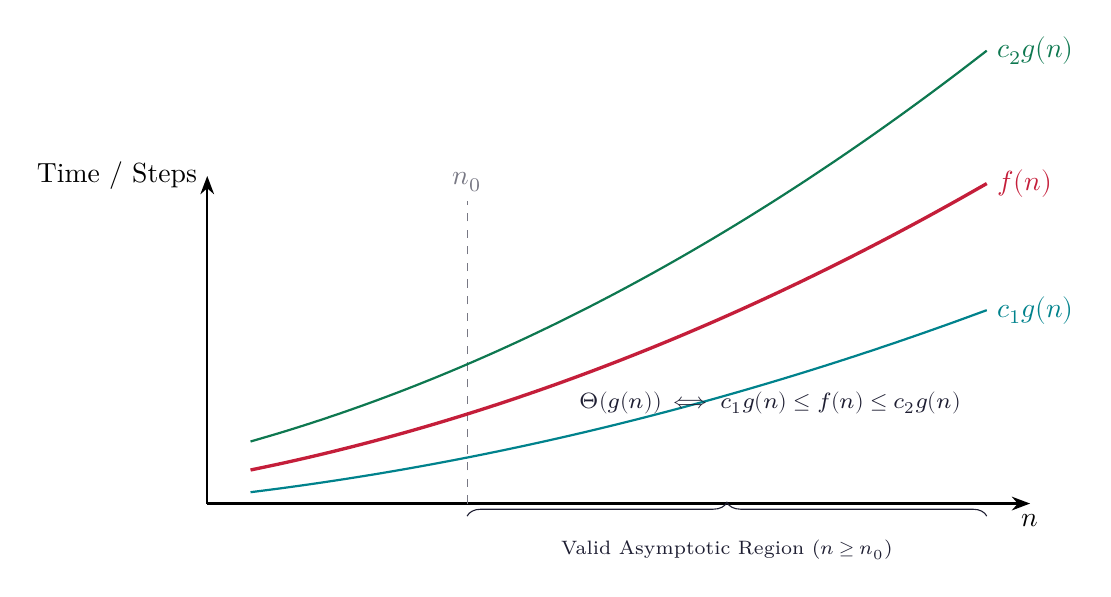
\begin{tikzpicture}[xscale=1.1, yscale=0.8]
  % Axes
  \draw[-Stealth, thick] (0,0) -- (9.5,0) node[below] {$n$};
  \draw[-Stealth, thick] (0,0) -- (0,5.2) node[left] {Time / Steps};

  % Threshold line n_0
  \draw[dashed, mydark!60] (3.0,0) -- (3.0,4.8) node[above] {$n_0$};

  % Big-Theta Curves
  \draw[domain=0.5:9, smooth, variable=\x, thick, color=mygreen] plot ({\x}, {0.35*\x + 0.04*\x*\x + 0.8}) node[right] {$c_2 g(n)$};
  \draw[domain=0.5:9, smooth, variable=\x, very thick, color=myred] plot ({\x}, {0.25*\x + 0.03*\x*\x + 0.4}) node[right] {$f(n)$};
  \draw[domain=0.5:9, smooth, variable=\x, thick, color=myteal] plot ({\x}, {0.15*\x + 0.02*\x*\x + 0.1}) node[right] {$c_1 g(n)$};

  % Shaded region
  \node[font=\footnotesize, color=mydark] at (6.5,1.6) {$\Theta(g(n)) \iff c_1 g(n) \le f(n) \le c_2 g(n)$};
  \draw[decorate, decoration={brace, amplitude=5pt}, mydark] (3.0,-0.2) -- (9.0,-0.2) node[midway, below=5pt, font=\scriptsize] {Valid Asymptotic Region ($n \ge n_0$)};
\end{tikzpicture}
\end{tcolorbox}

\subsection{Little-o and Little-omega Notations}
\begin{itemize}[leftmargin=*, itemsep=3pt]
  \item \textbf{Little-o Notation ($o$ --- Strict Upper Bound):}
  \begin{equation}
    f(n) = o(g(n)) \iff \lim_{n \to \infty} \frac{f(n)}{g(n)} = 0
  \end{equation}
  Unlike $\mathcal{O}$, $f(n)$ cannot be asymptotically equal to $g(n)$ (e.g., $2n = o(n^2)$, but $2n \ne o(n)$).
  \item \textbf{Little-omega Notation ($\omega$ --- Strict Lower Bound):}
  \begin{equation}
    f(n) = \omega(g(n)) \iff \lim_{n \to \infty} \frac{f(n)}{g(n)} = \infty
  \end{equation}
\end{itemize}

\subsection{Hierarchy and Properties of Growth Rates}
Standard asymptotic complexities scale monotonically:
\begin{align}
  \mathcal{O}(1) &< \mathcal{O}(\log \log n) < \mathcal{O}(\log n) < \mathcal{O}(\sqrt{n}) < \mathcal{O}(n) \notag\\
  &< \mathcal{O}(n \log n) < \mathcal{O}(n^2) < \mathcal{O}(n^3) < \mathcal{O}(2^n) < \mathcal{O}(n!) < \mathcal{O}(n^n)
\end{align}

\par\vspace{4pt}\noindent
\textbf{Fundamental Algebraic Properties:}
\begin{itemize}[leftmargin=*, itemsep=2pt]
  \item \textbf{Transitivity:} If $f(n) = \Theta(g(n))$ and $g(n) = \Theta(h(n))$, then $f(n) = \Theta(h(n))$.
  \item \textbf{Symmetry:} $f(n) = \Theta(g(n)) \iff g(n) = \Theta(f(n))$.
  \item \textbf{Transpose Symmetry:} $f(n) = \mathcal{O}(g(n)) \iff g(n) = \Omega(f(n))$.
  \item \textbf{Theorem:} $f(n) = \Theta(g(n)) \iff f(n) = \mathcal{O}(g(n)) \text{ and } f(n) = \Omega(g(n))$.
\end{itemize}

\subsection{The Time-Space Trade-Off}
In computational engineering, the \textbf{Time-Space Trade-off} dictates that algorithmic runtime can often be reduced at the expense of higher auxiliary memory usage, and vice-versa.
\begin{itemize}[leftmargin=*, itemsep=3pt]
  \item \textbf{Memory-Heavy, Fast Execution:} Hash tables provide $\mathcal{O}(1)$ average lookup by utilizing extra array buckets. Pre-computed lookup tables or memoization arrays in Dynamic Programming trade space to eliminate redundant exponential recursive calls.
  \item \textbf{Memory-Light, Slow Execution:} In-place algorithms with $\mathcal{O}(1)$ auxiliary space (e.g., linear scanning or recomputing values on demand) save RAM at the cost of $\mathcal{O}(n)$ or $\mathcal{O}(n^2)$ processing delays.
\end{itemize}

% ───────────────────────────────────────────────────────────────────────────────
\section{Searching Techniques and Algorithmic Complexity}
% ───────────────────────────────────────────────────────────────────────────────

\subsection{Linear (Sequential) Search}
Linear search scans an unsorted array sequentially from index $0$ to $n-1$, checking each element against target key $K$.

\begin{tcolorbox}[formulabox, title={\textbf{Linear Search Algorithm and Complexity Proof}}]
\textbf{Algorithm LinearSearch($A, n, K$):}
\begin{enumerate}[leftmargin=*, nosep]
  \item For $i = 0$ to $n - 1$ do:
  \item \quad If $A[i] == K$, return index $i$.
  \item Return $-1$ (Search Key Not Found).
\end{enumerate}
\par\vspace{4pt}\noindent
\textbf{Complexity Derivation:}
\begin{itemize}[leftmargin=*, itemsep=2pt]
  \item \textbf{Best-Case Time Complexity:} Target key is at the first index ($A[0] == K$). Requires $1$ comparison:
  \begin{equation}
    T_{\text{best}}(n) = \mathcal{O}(1)
  \end{equation}
  \item \textbf{Worst-Case Time Complexity:} Target key is at the last index ($A[n-1]$) or absent from array. Requires $n$ comparisons:
  \begin{equation}
    T_{\text{worst}}(n) = \mathcal{O}(n)
  \end{equation}
  \item \textbf{Average-Case Time Complexity:} Assuming uniform distribution where key is present with probability $p$, and equally likely at any position ($1/n$):
  \begin{equation}
    T_{\text{avg}}(n) = \sum_{i=1}^n i \cdot P(\text{found at } i) = \sum_{i=1}^n i \cdot \frac{1}{n} = \frac{1}{n} \cdot \frac{n(n+1)}{2} = \frac{n+1}{2} \implies \mathcal{O}(n)
  \end{equation}
  \item \textbf{Auxiliary Space:} $\mathcal{O}(1)$ (in-place search).
\end{itemize}
\end{tcolorbox}

\subsection{Binary Search Technique}
Binary search operates on a \textbf{monotonically sorted} contiguous sequence via divide-and-conquer, halving the search space in each iteration.

\begin{tcolorbox}[defbox, title={\textbf{Binary Search Algorithm (Iterative Implementation)}}]
\textbf{Algorithm BinarySearch($A, n, K$):}
\begin{enumerate}[leftmargin=*, nosep]
  \item Set $\text{low} = 0, \; \text{high} = n - 1$.
  \item While $\text{low} \le \text{high}$ do:
  \item \quad Compute $\text{mid} = \text{low} + \lfloor (\text{high} - \text{low})/2 \rfloor$. \quad \textit{(Prevents integer overflow)}
  \item \quad If $A[\text{mid}] == K$, return $\text{mid}$ (Success).
  \item \quad Else if $A[\text{mid}] < K$, set $\text{low} = \text{mid} + 1$.
  \item \quad Else set $\text{high} = \text{mid} - 1$.
  \item Return $-1$ (Key Absent).
\end{enumerate}
\end{tcolorbox}

\begin{tcolorbox}[tikzbox, title={\textbf{Decision Tree Representation of Binary Search on $n=7$ Elements}}]
\centering
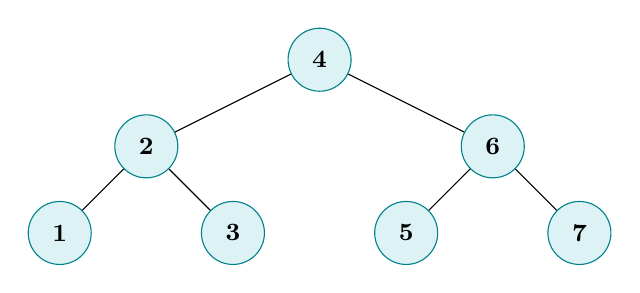
\begin{tikzpicture}[
  level distance=1.1cm,
  level 1/.style={sibling distance=4.4cm},
  level 2/.style={sibling distance=2.2cm},
  every node/.style={circle, draw=myteal, fill=hdrteal, font=\small\bfseries, inner sep=2pt, minimum size=0.8cm}
]
  \node {4}
    child { node {2}
      child { node {1} }
      child { node {3} }
    }
    child { node {6}
      child { node {5} }
      child { node {7} }
    };
\end{tikzpicture}
\par\vspace{2pt}
{\footnotesize At each stage, one comparison reduces the remaining search tree depth by 1. Total depth is $\lfloor \log_2 n \rfloor + 1$.}
\end{tcolorbox}

\begin{tcolorbox}[formulabox, title={\textbf{Binary Search Recurrence Relation and Complexity Derivation}}]
In each step, the algorithm performs $\mathcal{O}(1)$ comparisons and reduces problem size $n$ to $n/2$:
\begin{equation}
  T(n) = T\left(\frac{n}{2}\right) + c, \qquad T(1) = 1
\end{equation}
\textbf{Solving via Repeated Substitution (Unfolding):}
\begin{align*}
  T(n) &= T\left(\frac{n}{2}\right) + c = \left[T\left(\frac{n}{4}\right) + c\right] + c = T\left(\frac{n}{2^2}\right) + 2c \\
       &= T\left(\frac{n}{2^k}\right) + k \cdot c
\end{align*}
The process terminates when the subproblem reaches size 1: $\frac{n}{2^k} = 1 \implies 2^k = n \implies k = \log_2 n$.
\begin{equation}
  T(n) = T(1) + c \cdot \log_2 n = 1 + c \log_2 n \implies \mathbf{\Theta(\log_2 n)}
\end{equation}
\par\vspace{2pt}\noindent
\textbf{Summary of Bounds:}
\begin{itemize}[leftmargin=*, nosep]
  \item \textbf{Best-Case:} $A[\text{mid}] == K$ on first comparison $\implies \mathbf{\mathcal{O}(1)}$.
  \item \textbf{Worst-Case:} Element is at the leaf of the decision tree or absent $\implies \mathbf{\mathcal{O}(\log_2 n)}$.
  \item \textbf{Average-Case:} Successful search across all decision tree nodes $\implies \mathbf{\mathcal{O}(\log_2 n)}$.
  \item \textbf{Space Complexity:} $\mathcal{O}(1)$ for iterative version; $\mathcal{O}(\log_2 n)$ stack frames for recursive version.
\end{itemize}
\end{tcolorbox}

\subsection{Comparison: Linear Search vs Binary Search}
\par\vspace{6pt}\noindent
\begingroup
\setlength{\tabcolsep}{4.5pt}
\setlength{\extrarowheight}{3pt}
\renewcommand{\arraystretch}{1.35}
\begin{tabularx}{\linewidth}{|B{3.2cm}|Y|Y|}
\hline
\textbf{Criterion} & \textbf{Linear Search} & \textbf{Binary Search} \\
\hline
Prerequisite & Elements can be arbitrary/unsorted & Sequence \textbf{must} be monotonically sorted \\
\hline
Access Requirement & Sequential or Random access (Array or Linked List) & Random access required (Arrays only; inefficient on linked lists) \\
\hline
Best-Case Time & $\mathcal{O}(1)$ (first item matches) & $\mathcal{O}(1)$ (middle item matches) \\
\hline
Worst-Case Time & $\mathcal{O}(n)$ & $\mathcal{O}(\log_2 n)$ \\
\hline
Average-Case Time & $\mathcal{O}(n)$ & $\mathcal{O}(\log_2 n)$ \\
\hline
Space Complexity & $\mathcal{O}(1)$ in-place & $\mathcal{O}(1)$ iterative, $\mathcal{O}(\log n)$ recursive \\
\hline
Hardware Efficiency & Excellent CPU cache spatial locality & Multiple cache misses on large data jumps \\
\hline
Algorithm Paradigm & Brute-force linear scan & Divide-and-Conquer \\
\hline
\end{tabularx}
\endgroup

\newpage
% ===============================================================================
% MANDATORY QUICK REVISION PAGE
% ===============================================================================
\begin{center}
  {\large\bfseries\color{myred} Quick Revision --- Module 1}\\[3pt]
  {\small\color{mydark} Introduction, Algorithm Analysis and Searching Techniques $|$ ES-CS301}
\end{center}
\noindent{\color{myred}\rule{\linewidth}{1.2pt}}
\vspace{4pt}

\begin{tcolorbox}[formulabox, title={\textbf{Key Formulas and Asymptotic Relations at a Glance}}]
\renewcommand{\arraystretch}{1.25}
\begin{tabularx}{\linewidth}{B{5.0cm} X}
1D Array Address & $\text{Loc}(A[i]) = B + W \cdot (i - LB)$ \\[2pt]
2D Row-Major Address & $\text{Loc}(A[i][j]) = B + W \cdot [(i - LB_1) \cdot N_2 + (j - LB_2)]$ \\[2pt]
2D Column-Major Address & $\text{Loc}(A[i][j]) = B + W \cdot [(j - LB_2) \cdot N_1 + (i - LB_1)]$ \\[2pt]
Asymptotic Bounds ($\mathcal{O}, \Omega, \Theta$) & $f(n) \le c_1 g(n) \;(\mathcal{O}), \quad c_2 g(n) \le f(n) \;(\Omega), \quad c_3 g(n) \le f(n) \le c_4 g(n) \;(\Theta)$ \\[2pt]
Strict Limits ($o, \omega$) & $\lim_{n \to \infty} \frac{f(n)}{g(n)} = 0 \;(o), \quad \lim_{n \to \infty} \frac{f(n)}{g(n)} = \infty \;(\omega)$ \\[2pt]
Binary Search Recurrence & $T(n) = T(n/2) + \Theta(1) \implies T(n) = \Theta(\log_2 n)$ \\[2pt]
Linear Search Bounds & $\text{Best-Case: } \mathcal{O}(1), \quad \text{Worst-Case / Average: } \mathcal{O}(n)$ \\[2pt]
Complexity Hierarchy & $\mathcal{O}(1) < \mathcal{O}(\log n) < \mathcal{O}(n) < \mathcal{O}(n \log n) < \mathcal{O}(n^2) < \mathcal{O}(2^n) < \mathcal{O}(n!)$ \\[2pt]
\end{tabularx}
\end{tcolorbox}

\begin{tcolorbox}[defbox, title={\textbf{One-Line Definitions}}]
\begin{itemize}[leftmargin=*, itemsep=2pt, topsep=0pt]
  \item \textbf{Data Structure:} A logical and mathematical organization of data elements along with designated legal operations.
  \item \textbf{Abstract Data Type (ADT):} A mathematical model for data types defining behavior from user perspective without implementation details.
  \item \textbf{Linear Data Structure:} A data structure where elements form an ordered sequential sequence with 1-to-1 adjacent relations.
  \item \textbf{Row-Major Order (RMO):} A 2D mapping layout where all elements of row $i$ precede row $i+1$ in contiguous physical memory.
  \item \textbf{Column-Major Order (CMO):} A 2D mapping layout where all elements of column $j$ precede column $j+1$ in contiguous physical memory.
  \item \textbf{Big-O ($\mathcal{O}$):} An asymptotic notation defining a formal mathematical upper bound on algorithm computational growth.
  \item \textbf{Time-Space Trade-off:} The engineering principle where computational runtime is decreased by allocating extra memory.
  \item \textbf{Binary Search:} A divide-and-conquer algorithm on sorted arrays halving search space in $\mathcal{O}(\log_2 n)$ comparisons.
\end{itemize}
\end{tcolorbox}

\newpage

\begin{tcolorbox}[exambox, title={\textbf{Frequently Asked / Viva Questions (Part 1)}}]
\begin{enumerate}[topsep=0pt, label=\textbf{Q\arabic*.}, itemsep=4pt]
  \item \Q{What is the difference between a Data Type and a Data Structure?}
  A data type is a primitive classification defining a set of values and allowable low-level hardware operations (e.g., \texttt{int}, \texttt{float}). A data structure is a higher-level collection of data elements organized logically with specific algorithms to store and manipulate them efficiently in memory (e.g., arrays, stacks, trees).

  \item \Q{Why do we prefer asymptotic notations over clock time for analyzing algorithms?}
  Physical clock time depends on machine architecture, processor speed, compiler optimizations, background processes, and cache memory. Asymptotic notations evaluate performance purely as a function of input size $n$, independent of hardware, providing an objective, universal measure of scalability.

  \item \Q{State the necessary and sufficient condition for $f(n) = \Theta(g(n))$.}
  The function $f(n) = \Theta(g(n))$ if and only if $f(n) = \mathcal{O}(g(n))$ and $f(n) = \Omega(g(n))$. That is, $g(n)$ serves simultaneously as both the asymptotic upper bound and lower bound within positive constant multipliers $c_1$ and $c_2$.

  \item \Q{Why must an array be sorted prior to executing Binary Search?}
  Binary search relies on the monotonicity of elements. When the target key $K$ is compared with the middle element $A[\text{mid}]$, the algorithm assumes that all elements to the left are $\le A[\text{mid}]$ and all elements to the right are $\ge A[\text{mid}]$. Without sorted order, discarding half the array could eliminate the target key.

  \item \Q{Why is Binary Search inefficient when applied to a Singly Linked List?}
  Binary search requires finding the midpoint in $\mathcal{O}(1)$ time. In a linked list, random access is not supported ($A[i]$ takes $\mathcal{O}(i)$ traversal steps). Locating the middle node takes $\mathcal{O}(n)$ time, which negates the divide-and-conquer speedup, resulting in overall $\mathcal{O}(n)$ complexity.

  \item \Q{Explain the concept of integer overflow in computing the midpoint in Binary Search and how it is resolved.}
  Writing \texttt{mid = (low + high) / 2} can cause integer overflow if the sum \texttt{low + high} exceeds the maximum 32-bit signed integer value ($2^{31}-1$). The overflow wraps to a negative number, causing an index out-of-bounds fault. It is avoided using \texttt{mid = low + (high - low) / 2}.

  \item \Q{Differentiate between Big-O ($\mathcal{O}$) and Little-o ($o$).}
  Big-O establishes an asymptotic upper bound that may be tight ($2n^2 = \mathcal{O}(n^2)$ is valid). Little-o establishes a strict, non-tight upper bound such that $f(n)$ grows strictly slower than $g(n)$ as $n \to \infty$ ($\lim_{n \to \infty} f(n)/g(n) = 0$). Thus $2n = o(n^2)$, but $2n^2 \ne o(n^2)$.
\end{enumerate}
\end{tcolorbox}

\newpage

\begin{tcolorbox}[exambox, title={\textbf{Frequently Asked / Viva Questions (Part 2)}}]
\begin{enumerate}[topsep=0pt, label=\textbf{Q\arabic*.}, itemsep=4pt, start=8]
  \item \Q{What is the difference between Space Complexity and Auxiliary Space?}
  Space complexity is the total memory used by an algorithm, including both the input data and any extra working memory. Auxiliary space refers exclusively to the extra temporary or scratchpad memory allocated by the algorithm beyond the input size.

  \item \Q{Provide an example of an engineering Time-Space trade-off.}
  In calculating Fibonacci numbers: naive recursion takes $\mathcal{O}(2^n)$ time and $\mathcal{O}(n)$ call-stack space. Using dynamic programming memoization with an auxiliary array of size $n$, runtime drops dramatically to $\mathcal{O}(n)$ time at the expense of $\mathcal{O}(n)$ extra storage space.

  \item \Q{What are the worst-case, best-case, and average-case scenarios for Linear Search?}
  Best case is $\mathcal{O}(1)$ (element found at index $0$). Worst case is $\mathcal{O}(n)$ (element is at index $n-1$ or absent). Average case is $\mathcal{O}(n)$ (specifically $(n+1)/2$ comparisons under a uniform random distribution).
\end{enumerate}
\end{tcolorbox}

\vspace{3pt}

\begin{tcolorbox}[tikzbox, title={\textbf{Summary Matrix: Comprehensive Comparison of Searching and Analysis Fundamentals}}]
\par\vspace{2pt}\noindent
\begingroup
\footnotesize
\setlength{\tabcolsep}{3.5pt}
\setlength{\extrarowheight}{1.5pt}
\renewcommand{\arraystretch}{1.15}
\begin{tabularx}{\linewidth}{|B{2.4cm}|B{3.2cm}|B{2.8cm}|Y|}
\hline
\textbf{Topic / Technique} & \textbf{Core Governing Relation} & \textbf{Complexity Bound} & \textbf{Key Engineering Takeaway} \\
\hline
Row-Major 2D Addressing & $\text{Loc} = B + W[(i-LB_1)N_2 + (j-LB_2)]$ & $\mathcal{O}(1)$ compute time & C/C++ memory layout; row iteration preserves cache locality. \\
\hline
Column-Major 2D Addressing & $\text{Loc} = B + W[(j-LB_2)N_1 + (i-LB_1)]$ & $\mathcal{O}(1)$ compute time & Fortran/MATLAB layout; column-by-column iteration preferred. \\
\hline
Big-O Notation ($\mathcal{O}$) & $f(n) \le c \cdot g(n) \;\; \forall n \ge n_0$ & Upper bound & Worst-case computational ceiling guarantees. \\
\hline
Big-Theta Notation ($\Theta$) & $c_1 g(n) \le f(n) \le c_2 g(n)$ & Tight bound & Exact algorithmic rate of growth. \\
\hline
Linear Search & Sequential traversal $A[0 \dots n-1]$ & Worst: $\mathcal{O}(n)$, Best: $\mathcal{O}(1)$ & Unsorted or small lists; works natively on linked lists. \\
\hline
Binary Search & $T(n) = T(n/2) + \mathcal{O}(1)$ & Worst: $\mathcal{O}(\log n)$, Best: $\mathcal{O}(1)$ & Strictly requires sorted array and random access memory. \\
\hline
\end{tabularx}
\endgroup
\end{tcolorbox}

\end{document}
